%======================================================================
% University of Waterloo Thesis Template for LaTeX 
% Last Updated August 2023
% by IST Client Services, 
% University of Waterloo, 200 University Ave. W., Waterloo, Ontario, Canada
% FOR ASSISTANCE, please send mail to ist-helpdesk@uwaterloo.ca

% DISCLAIMER
% To the best of our knowledge, this template satisfies the current uWaterloo thesis requirements.
% However, it is your responsibility to assure that you have met all requirements of the University and your particular department.

% Many thanks for the feedback from many graduates who assisted the development of this template.
% Also note that there are explanatory comments and tips throughout this template.
%======================================================================
% Some important notes on using this template and making it your own...

% The University of Waterloo has required electronic thesis submission since October 2006. 
% See the uWaterloo thesis regulations at
% https://uwaterloo.ca/graduate-studies/thesis.
% This thesis template is geared towards generating a PDF version optimized for viewing on an electronic display, including hyperlinks within the PDF.

% DON'T FORGET TO ADD YOUR OWN NAME AND TITLE in the "hyperref" package configuration below. 
% Search for: PDFTITLE, PDFAUTHOR, PDFSUBJECT, and PDFKEYWORDS.
% THIS INFORMATION GETS EMBEDDED IN THE FINAL PDF DOCUMENT.
% You can view the information if you view properties of the PDF document.

% Many faculties/departments also require one or more printed copies. 
% This template attempts to satisfy both types of output. 
% See additional notes below.
% It is based on the standard "book" document class which provides all necessary sectioning structures and allows multi-part theses.

% If you are using this template in Overleaf (cloud-based collaboration service), then it is automatically processed and previewed for you as you edit.

% For people who prefer to install their own LaTeX distributions on their own computers, and process the source files manually, the following notes provide the sequence of tasks:
 
% E.g. to process a thesis called "mythesis.tex" based on this template, run:

% pdflatex mythesis	-- first pass of the pdflatex processor
% bibtex mythesis	-- generates bibliography from .bib data file(s)
% makeindex         -- should be run only if an index is used 
% pdflatex mythesis	-- fixes numbering in cross-references, bibliographic references, glossaries, index, etc.
% pdflatex mythesis	-- it takes a couple of passes to completely process all cross-references

% If you use the recommended LaTeX editor, Texmaker, you would open the mythesis.tex file, then click the PDFLaTeX button. Then run BibTeX (under the Tools menu).
% Then click the PDFLaTeX button two more times. 
% If you have an index as well,you'll need to run MakeIndex from the Tools menu as well, before running pdflatex
% the last two times.

% N.B. The "pdftex" program allows graphics in the following formats to be included with the "\includegraphics" command: PNG, PDF, JPEG, TIFF
% Tip: Generate your figures and photos in the size you want them to appear in your thesis, rather than scaling them with \includegraphics options.
% Tip: Any drawings you do should be in scalable vector graphic formats: SVG, PNG, WMF, EPS and then converted to PNG or PDF, so they are scalable in the final PDF as well.
% Tip: Photographs should be cropped and compressed so as not to be too large.

% To create a PDF output that is optimized for double-sided printing: 
% 1) comment-out the \documentclass statement in the preamble below, and un-comment the second \documentclass line.
% 2) change the value assigned below to the boolean variable "PrintVersion" from " false" to "true".

%======================================================================
%   D O C U M E N T   P R E A M B L E
% Specify the document class, default style attributes, and page dimensions, etc.
% For hyperlinked PDF, suitable for viewing on a computer, use this:
\documentclass[letterpaper,12pt,titlepage,oneside,final]{book}
 
% For PDF, suitable for double-sided printing, change the PrintVersion variable below to "true" and use this \documentclass line instead of the one above:
%\documentclass[letterpaper,12pt,titlepage,openright,twoside,final]{book}

% Some LaTeX commands I define for my own nomenclature.
% If you have to, it's easier to make changes to nomenclature once here than in a million places throughout your thesis!
\newcommand{\package}[1]{\textbf{#1}} % package names in bold text
\newcommand{\cmmd}[1]{\textbackslash\texttt{#1}} % command name in tt font 
\newcommand{\href}[1]{#1} % does nothing, but defines the command so the print-optimized version will ignore \href tags (redefined by hyperref pkg).
%\newcommand{\texorpdfstring}[2]{#1} % does nothing, but defines the command
% Anything defined here may be redefined by packages added below...

% This package allows if-then-else control structures.
\usepackage{ifthen}
\newboolean{PrintVersion}
\setboolean{PrintVersion}{false}
% CHANGE THIS VALUE TO "true" as necessary, to improve printed results for hard copies by overriding some options of the hyperref package, called below.

%\usepackage{nomencl} % For a nomenclature (optional; available from ctan.org)
\usepackage{amsmath,amssymb,amstext} % Lots of math symbols and environments
\usepackage[pdftex]{graphicx} % For including graphics N.B. pdftex graphics driver 

% Hyperlinks make it very easy to navigate an electronic document.
% In addition, this is where you should specify the thesis title and author as they appear in the properties of the PDF document.
% Use the "hyperref" package 
% N.B. HYPERREF MUST BE THE LAST PACKAGE LOADED; ADD ADDITIONAL PKGS ABOVE
\usepackage[pdftex,pagebackref=false]{hyperref} % with basic options
%\usepackage[pdftex,pagebackref=true]{hyperref}
		% N.B. pagebackref=true provides links back from the References to the body text. This can cause trouble for printing.
\hypersetup{
    plainpages=false,       % needed if Roman numbers in frontpages
    unicode=false,          % non-Latin characters in Acrobat’s bookmarks
    pdftoolbar=true,        % show Acrobat’s toolbar?
    pdfmenubar=true,        % show Acrobat’s menu?
    pdffitwindow=false,     % window fit to page when opened
    pdfstartview={FitH},    % fits the width of the page to the window
%    pdftitle={uWaterloo\ LaTeX\ Thesis\ Template},    % title: CHANGE THIS TEXT!
%    pdfauthor={Author},    % author: CHANGE THIS TEXT! and uncomment this line
%    pdfsubject={Subject},  % subject: CHANGE THIS TEXT! and uncomment this line
%    pdfkeywords={keyword1} {key2} {key3}, % list of keywords, and uncomment this line if desired
    pdfnewwindow=true,      % links in new window
    colorlinks=true,        % false: boxed links; true: colored links
    linkcolor=blue,         % color of internal links
    citecolor=green,        % color of links to bibliography
    filecolor=magenta,      % color of file links
    urlcolor=cyan           % color of external links
}
\ifthenelse{\boolean{PrintVersion}}{   % for improved print quality, change some hyperref options
\hypersetup{	% override some previously defined hyperref options
%    colorlinks,%
    citecolor=black,%
    filecolor=black,%
    linkcolor=black,%
    urlcolor=black}
}{} % end of ifthenelse (no else)

\usepackage[automake,toc,abbreviations]{glossaries-extra} % Exception to the rule of hyperref being the last add-on package
% If glossaries-extra is not in your LaTeX distribution, get it from CTAN (http://ctan.org/pkg/glossaries-extra), 
% although it's supposed to be in both the TeX Live and MikTeX distributions. There are also documentation and 
% installation instructions there.

% GYX: my packages
\usepackage{booktabs}
\usepackage{tikz}
\usetikzlibrary{calc}
\usetikzlibrary{positioning}

% GYX: custom commands
\newcommand{\pke}{\texttt{PKE}}
\newcommand{\keygen}{\texttt{KeyGen}}
\newcommand{\encrypt}{\texttt{Enc}}
\newcommand{\decrypt}{\texttt{Dec}}
\newcommand{\kem}{\texttt{KEM}}
\newcommand{\encap}{\texttt{Encap}}
\newcommand{\decap}{\texttt{Decap}}
\newcommand{\etm}{{\texttt{ETM}}}  % encrypt-then-mac
\newcommand{\mac}{\texttt{\texttt{MAC}}}
\newcommand{\sign}{\texttt{Sign}}
\newcommand{\verify}{\texttt{Verify}}
\newcommand{\pk}{\texttt{pk}}
\newcommand{\sk}{\texttt{sk}}
\newcommand{\pco}{\texttt{PCO}}
\newcommand{\cvo}{\texttt{CVO}}
\newcommand{\leftsample}{\stackrel{\$}{\leftarrow}}
\newcommand{\llbrack}{[\![}
\newcommand{\rrbrack}{]\!]}
\newcommand{\norm}[1]{\left\lvert #1 \right\rvert}
\newcommand{\adv}{\texttt{Adv}}
\newcommand{\fotplus}{\texttt{FOT+}}
\newcommand{\us}{\mu s}
\Urlmuskip=0mu  plus 10mu  % fix underfull hbox for URL in footnote

% Setting up the page margins...
% uWaterloo thesis requirements specify a minimum of 1 inch (72pt) margin at the
% top, bottom, and outside page edges and a 1.125 in. (81pt) gutter margin (on binding side). 
% While this is not an issue for electronic viewing, a PDF may be printed, and so we have the same page layout for both printed and electronic versions, we leave the gutter margin in.
% Set margins to minimum permitted by uWaterloo thesis regulations:
\setlength{\marginparwidth}{0pt} % width of margin notes
% N.B. If margin notes are used, you must adjust \textwidth, \marginparwidth
% and \marginparsep so that the space left between the margin notes and page
% edge is less than 15 mm (0.6 in.)
\setlength{\marginparsep}{0pt} % width of space between body text and margin notes
\setlength{\evensidemargin}{0.125in} % Adds 1/8 in. to binding side of all 
% even-numbered pages when the "twoside" printing option is selected
\setlength{\oddsidemargin}{0.125in} % Adds 1/8 in. to the left of all pages when "oneside" printing is selected, and to the left of all odd-numbered pages when "twoside" printing is selected
\setlength{\textwidth}{6.375in} % assuming US letter paper (8.5 in. x 11 in.) and side margins as above
\raggedbottom

% The following statement specifies the amount of space between paragraphs. Other reasonable specifications are \bigskipamount and \smallskipamount.
\setlength{\parskip}{\medskipamount}

% The following statement controls the line spacing.  
% The default spacing corresponds to good typographic conventions and only slight changes (e.g., perhaps "1.2"), if any, should be made.
\renewcommand{\baselinestretch}{1} % this is the default line space setting

% By default, each chapter will start on a recto (right-hand side) page.
% We also force each section of the front pages to start on a recto page by inserting \cleardoublepage commands.
% In many cases, this will require that the verso (left-hand) page be blank, and while it should be counted, a page number should not be printed.
% The following statements ensure a page number is not printed on an otherwise blank verso page.
\let\origdoublepage\cleardoublepage
\newcommand{\clearemptydoublepage}{%
  \clearpage{\pagestyle{empty}\origdoublepage}}
\let\cleardoublepage\clearemptydoublepage

% Define Glossary terms (This is properly done here, in the preamble and could also be \input{} from a separate file...)
% Main glossary entries -- definitions of relevant terminology
\newglossaryentry{computer}
{
name=computer,
description={A programmable machine that receives input data,
               stores and manipulates the data, and provides
               formatted output}
}

% Nomenclature glossary entries -- New definitions, or unusual terminology
\newglossary*{nomenclature}{Nomenclature}
\newglossaryentry{dingledorf}
{
type=nomenclature,
name=dingledorf,
description={A person of supposed average intelligence who makes incredibly brainless misjudgments}
}

% List of Abbreviations (abbreviations type is built in to the glossaries-extra package)
\newabbreviation{aaaaz}{AAAAZ}{American Association of Amateur Astronomers and Zoologists}

% List of Symbols
\newglossary*{symbols}{List of Symbols}
\newglossaryentry{rvec}
{
name={$\mathbf{v}$},
sort={label},
type=symbols,
description={Random vector: a location in n-dimensional Cartesian space, where each dimensional component is determined by a random process}
}
\makeglossaries

%======================================================================
%   L O G I C A L    D O C U M E N T
% The logical document contains the main content of your thesis.
% Being a large document, it is a good idea to divide your thesis into several files, each one containing one chapter or other significant chunk of content, so you can easily shuffle things around later if desired.
%======================================================================
\begin{document}

%----------------------------------------------------------------------
% FRONT MATERIAL
% title page, examining committee membership (for PhD Thesis only), declaration, borrowers' page, abstract, acknowledgements,
% dedication, table of contents, list of tables, list of figures, nomenclature, etc.
%----------------------------------------------------------------------
% T I T L E   P A G E
% -------------------
% Last updated August 24, 2023, by IST-Client Services
% The title page is counted as page `i' but we need to suppress the
% page number. Also, we don't want any headers or footers.
\pagestyle{empty}
\pagenumbering{roman}

% The contents of the title page are specified in the "titlepage"
% environment.
\begin{titlepage}
        \begin{center}
        \vspace*{1.0cm}

        \Huge
        {\bf University of Waterloo E-Thesis Template for \LaTeX }

        \vspace*{1.0cm}

        \normalsize
        by \\

        \vspace*{1.0cm}

        \Large
        Pat Neugraad \\

        \vspace*{3.0cm}

        \normalsize
        A thesis \\
        presented to the University of Waterloo \\ 
        in fulfillment of the \\
        thesis requirement for the degree of \\
        Doctor of Philosophy \\
        in \\
        Philosophy of Zoology \\

        \vspace*{2.0cm}

        Waterloo, Ontario, Canada, 2023 \\

        \vspace*{1.0cm}

        \copyright\ Pat Neugraad 2023 \\
        \end{center}
\end{titlepage}

% The rest of the front pages should contain no headers and be numbered using Roman numerals starting with `ii'
\pagestyle{plain}
\setcounter{page}{2}

\cleardoublepage % Ends the current page and causes all figures and tables that have so far appeared in the input to be printed.
% In a two-sided printing style, it also makes the next page a right-hand (odd-numbered) page, producing a blank page if necessary.
\phantomsection    % allows hyperref to link to the correct page
 
% E X A M I N I N G   C O M M I T T E E (Required for Ph.D. theses only)
% Remove or comment out the lines below to remove this page
\addcontentsline{toc}{chapter}{Examining Committee}
\begin{center}\textbf{Examining Committee Membership}\end{center}
  \noindent
The following served on the Examining Committee for this thesis. The decision of the Examining Committee is by majority vote.
  \bigskip
  
  \noindent
\begin{tabbing}
Internal-External Member: \=  \kill % using longest text to define tab length
External Examiner: \>  Bruce Bruce \\ 
\> Professor, Dept. of Philosophy of Zoology, University of Wallamaloo \\
\end{tabbing} 
  \bigskip
  
  \noindent
\begin{tabbing}
Internal-External Member: \=  \kill % using longest text to define tab length
Supervisor(s): \> Ann Elk \\
\> Professor, Dept. of Zoology, University of Waterloo \\
\> Andrea Anaconda \\
\> Professor Emeritus, Dept. of Zoology, University of Waterloo \\
\end{tabbing}
  \bigskip
  
  \noindent
  \begin{tabbing}
Internal-External Member: \=  \kill % using longest text to define tab length
Internal Member: \> Pamela Python \\
\> Professor, Dept. of Zoology, University of Waterloo \\
\end{tabbing}
  \bigskip
  
  \noindent
\begin{tabbing}
Internal-External Member: \=  \kill % using longest text to define tab length
Internal-External Member: \> Meta Meta \\
\> Professor, Dept. of Philosophy, University of Waterloo \\
\end{tabbing}
  \bigskip
  
  \noindent
\begin{tabbing}
Internal-External Member: \=  \kill % using longest text to define tab length
Other Member(s): \> Leeping Fang \\
\> Professor, Dept. of Fine Art, University of Waterloo \\
\end{tabbing}

\cleardoublepage
\phantomsection    % allows hyperref to link to the correct page

% D E C L A R A T I O N   P A G E
% -------------------------------
  % The following is a sample Declaration Page as provided by the GSPA
  % December 13th, 2006.  It is designed for an electronic thesis.
 \addcontentsline{toc}{chapter}{Author's Declaration}
 \begin{center}\textbf{Author's Declaration}\end{center}

 % Author's Declaration Option ONE - line 118:  
 \noindent
I hereby declare that I am the sole author of this thesis. This is a true copy of the thesis, including any required final revisions, as accepted by my examiners.
  % Author's Declaration Option TWO - line 121. Updated August 21st, 2023. Use the following declaration text if appropriate by removing the percent character and space at the beginning of line 121, and add a percent symbol and space at line 118 to change Author's Declaration Option ONE to a remark that is not printed.
 \noindent  
% This thesis consists of material all of which I authored or co-authored: see Statement of Contributions included in the thesis. This is a true copy of the thesis, including any required final revisions, as accepted by my examiners.
  \bigskip
  
  \noindent
I understand that my thesis may be made electronically available to the public.

\cleardoublepage
\phantomsection    % allows hyperref to link to the correct page

% A B S T R A C T
% ---------------
\addcontentsline{toc}{chapter}{Abstract}
\begin{center}\textbf{Abstract}\end{center}

This is the abstract.


\cleardoublepage
\phantomsection    % allows hyperref to link to the correct page

% A C K N O W L E D G E M E N T S
% -------------------------------
\addcontentsline{toc}{chapter}{Acknowledgements}
\begin{center}\textbf{Acknowledgements}\end{center}

I would like to thank all the little people who made this thesis possible.
\cleardoublepage
\phantomsection    % allows hyperref to link to the correct page

% D E D I C A T I O N
% -------------------
\addcontentsline{toc}{chapter}{Dedication}
\begin{center}\textbf{Dedication}\end{center}

This is dedicated to the one I love.
\cleardoublepage
\phantomsection    % allows hyperref to link to the correct page

% T A B L E   O F   C O N T E N T S
% ---------------------------------
\renewcommand\contentsname{Table of Contents}
\tableofcontents
\cleardoublepage
\phantomsection    % allows hyperref to link to the correct page

% L I S T   O F   F I G U R E S
% -----------------------------
\addcontentsline{toc}{chapter}{List of Figures}
\listoffigures
\cleardoublepage
\phantomsection		% allows hyperref to link to the correct page

% L I S T   O F   T A B L E S
% ---------------------------
\addcontentsline{toc}{chapter}{List of Tables}
\listoftables
\cleardoublepage
\phantomsection		% allows hyperref to link to the correct page

% L I S T   O F   A B B R E V I A T I O N S
% ---------------------------
\renewcommand*{\abbreviationsname}{List of Abbreviations}
\printglossary[type=abbreviations]
\cleardoublepage
\phantomsection		% allows hyperref to link to the correct page

% L I S T   O F   S Y M B O L S
% ---------------------------
\printglossary[type=symbols]
\cleardoublepage
\phantomsection		% allows hyperref to link to the correct page


% Change page numbering back to Arabic numerals
\pagenumbering{arabic}

\chapter{Post-quantum TLS on embedded systems}
\section{An overview of TLS 1.3}
Transport Layer Security (TLS) is a communication protocol with which two parties can securely exchange data over an insecure transport layer.
It was first developed at Netscape in 1994 and went through many iterations.
The latest revision is TLS 1.3, formally standardized by IETF in RFC8446 \cite{DBLP:journals/rfc/rfc8446} in 2018.
TLS 1.3 made significant improvements over TLS 1.2 \cite{DBLP:journals/rfc/rfc5246} and prior versions, including deprecating weak symmetric cipher suites, removing static key exchange schemes that do not provide forward secrecy, and restructuring the handshake state machine in order to simplify the handshake workflow.
According to Cloudflare \cite{Westerbaan_2024}, TLS 1.3 reached more than 93\% adoption on the Internet.
Given TLS 1.3's superior design and nearly universal adoption over other versions of TLS, this work will focus on this version unless otherwise specified.

A new TLS 1.3 connection begins with a handshake in which the two parties exchange a specific sequence of messages to negotiate cryptographic parameters, establish shared secrets, and authenticate each other.
If the handshake is successful, then the connection transitions to exchanging application data using the encryption scheme and secret keys obtained from the handshake phase.
In TLS 1.3, the handshake can be further divided into two phases \footnote{We omitted parameter negotiation messages like \texttt{HelloRetryRequest} and \texttt{EncryptedExtensions}. They are either optional or inconsequential to our argument}: \begin{enumerate}
    \item \textbf{Key exchange} \begin{enumerate}
        \item \texttt{ClientHello}: client publishes its supported symmetric cipher suites (AEAD, hash functions), signature algorithms, a random nonce, and key exchange public keys.
        \item \texttt{ServerHello}: server chooses its preferred symmetric cipher suite, as well as publishes its own random nonce and key exchange public keys.
    \end{enumerate}
    \item \textbf{Authentication} \begin{enumerate}
        \item \texttt{Certificates}: server sends a chain of X.509 certificates that bind its identity to a digital signature public key; optionally, server can request client authentication (\texttt{CertificateRequest}), in which case the client must also send a chain of certificates.
        \item \texttt{CertificatesVerify}: server proves ownership fo the corresponding digital signature secret key by producing a signature over the handshake transcript; client will do the same upon server's request
        \item \texttt{Finished}: both parties prove to each other the integrity of the handshake by producing an HMAC over the handshake transcript
    \end{enumerate}
\end{enumerate}

Figure \ref{fig:classical-tls13-handshake} illustrates a simple TLS 1.3 handshake:

\begin{figure}[htbp]
    \centering
    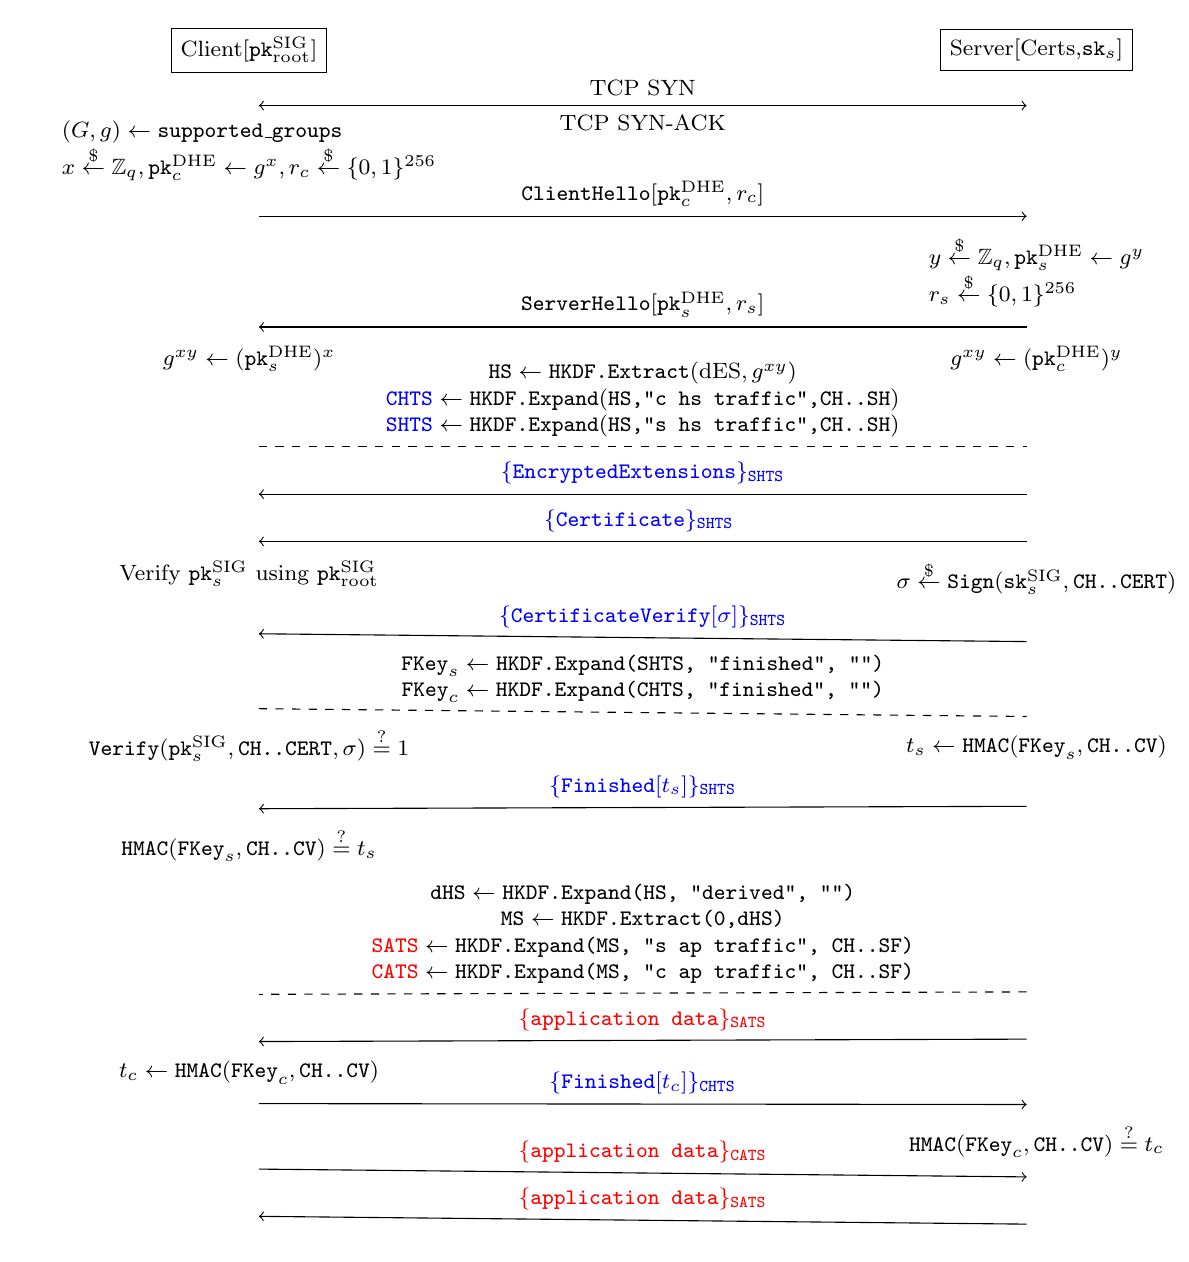
\begin{tikzpicture}[node distance=2em and 2.5cm, font=\footnotesize]
        \tikzset{
            mynode/.style = {draw, rectangle}
        }
    
        \node[draw,rectangle] (client) at (0,0) {Client[$\pk^\text{SIG}_\text{root}$]};
        \node[draw,rectangle] (server) at (10,0) {
            Server[Certs,$\sk_s$]
        };

        \node[below of=client] (tcpc) {}; % invisible nodes help draw TCP connection
        \node[below of=server] (tcps) {};
        \draw[<->] (tcpc) -- (tcps) node[midway,above]{TCP SYN} node[midway,below]{TCP SYN-ACK};

        % construct ClientHello
        \node[below of=tcpc,align=left] (ch) {
            $(G, g) \leftarrow \texttt{supported\_groups}$ \\
            $x \leftsample \mathbb{Z}_q,\pk^\text{DHE}_c\leftarrow g^x,r_c \leftsample \{0,1\}^{256}$ \\
        };
        \node[below of=tcps] (ch_wait) {}; % server is waiting for client hello

        % send ClientHello
        \node[below of=ch] (ch_sent) {};
        \node[below of=ch_wait] (ch_recved) {};
        \draw[->] (ch_sent) -- (ch_recved) node[midway,above] {\texttt{ClientHello}[$\pk^\text{DHE}_c,r_c$]};

        % process client hello, construct server hello
        \node[below of=ch_sent] (sh_wait) {};
        \node[align=left,below of=ch_recved] (sh) {
            $y\leftsample \mathbb{Z}_q,\pk^\text{DHE}_s\leftarrow g^y$ \\
            $r_s\leftsample\{0,1\}^{256}$
        };

        % send server hello
        \node[below of=sh_wait] (sh_recved) {};
        \node[below of=sh] (sh_sent) {};
        \draw[->] (sh_sent) -- (sh_recved) node[midway,above] {
            \texttt{ServerHello}[$\pk^\text{DHE}_s, r_s$]
        };

        % derive stage 1/2 keys: handshake traffic keys
        \node[align=left,below=0em of sh_recved] (dhe_ss_c) {$g^{xy}\leftarrow (\pk^\text{DHE}_s)^x$};
        \node[below=0em of sh_sent] (dhe_ss_s) {$g^{xy}\leftarrow (\pk^\text{DHE}_c)^y$};
        \node[below=2em of dhe_ss_c] (stage12_c) {};
        \node[below=2em of dhe_ss_s] (stage12_s) {};
        \draw[dashed] (stage12_c) -- (stage12_s) node[midway,above,align=center] {
            $\texttt{HS}\leftarrow\texttt{HKDF.Extract}(\text{dES}, g^{xy})$ \\
            $\texttt{\color{blue} CHTS} \leftarrow \texttt{HKDF.Expand}(\texttt{HS,"c hs traffic",CH..SH})$ \\
            $\texttt{\color{blue} SHTS} \leftarrow \texttt{HKDF.Expand}(\texttt{HS,"s hs traffic",CH..SH})$
        };

        % encrypted extensions, aka server parameters
        \node[below=1em of stage12_c] (serverparams_c) {};
        \node[below=1em of stage12_s] (serverparams_s) {};
        \draw[->] (serverparams_s) -- (serverparams_c) node[midway,above] {\color{blue}
            $\{\texttt{EncryptedExtensions}\}_\texttt{SHTS}$
        };

        % certificates
        \node[below=1em of serverparams_c] (certs_recv) {};
        \node[below=1em of serverparams_s] (certs_send) {};
        \draw[->] (certs_send) -- (certs_recv) node[midway,above,align=center] {\color{blue}
            $\{\texttt{Certificate}\}_\texttt{SHTS}$
        };

        % construct CertificateVerify
        \node[below=0em of certs_recv] (cv_wait) {
            Verify $\pk^\text{SIG}_s$ using 
            $\pk^\text{SIG}_\text{root}$
        };
        \node[below=0em of certs_send] (cv) {
            $\sigma \leftsample \sign(\sk^\text{SIG}_s, \texttt{CH..CERT})$
        };

        % send CertificateVerify
        \node[below=1em of cv_wait] (cv_recv) {
        };
        \node[below=1em of cv] (cv_send) {
        };
        \draw[->] (cv_send) -- (cv_recv) node[midway,above] {\color{blue}
            $\{\texttt{CertificateVerify}[\sigma]\}_\texttt{SHTS}$
        };

        % derive finished keys
        \node[below=2em of cv_recv] (finkey_c) {};
        \node[below=2em of cv_send] (finkey_s) {};
        \draw[dashed] (finkey_c) -- (finkey_s) node[midway,above,align=center] {
            $\texttt{FKey}_s \leftarrow \texttt{HKDF.Expand(SHTS, "finished", "")}$ \\
            $\texttt{FKey}_c \leftarrow \texttt{HKDF.Expand(CHTS, "finished", "")}$
        };

        % construct server finished
        \node[below=0em of finkey_c] (sfin_wait) {
            $\verify(\pk^\text{SIG}_s, \texttt{CH..CERT}, \sigma) \stackrel{?}{=} 1$
        };
        \node[below=0em of finkey_s] (sfin) {
            $t_s \leftarrow \texttt{HMAC}(\texttt{FKey}_s, \texttt{CH..CV})$
        };

        % send server finished
        \node[below=1em of sfin_wait] (sfin_recv) {};
        \node[below=1em of sfin] (sfin_send) {};
        \draw[->] (sfin_send) -- (sfin_recv) node[midway,above] {\color{blue}
            $\{\texttt{Finished}[t_s]\}_\texttt{SHTS}$
        };

        % client verified ServerFinished
        \node[below=0em of sfin_recv] (sfin_verify) {
            $\texttt{HMAC}(\texttt{FKey}_s, \texttt{CH..CV}) \stackrel{?}{=} t_s$
        };

        % derive MS, app traffic keys
        \node[below=6em of sfin_recv] (stage34_c) {};
        \node[below=6em of sfin_send] (stage34_s) {};
        \draw[dashed] (stage34_s) -- (stage34_c) node[midway,above,align=center] {
            $\texttt{dHS} \leftarrow \texttt{HKDF.Expand(HS, "derived", "")}$ \\
            $\texttt{MS} \leftarrow \texttt{HKDF.Extract(0,dHS)}$ \\
            $\texttt{\color{red} SATS} \leftarrow \texttt{HKDF.Expand(MS, "s ap traffic", CH..SF)}$ \\
            $\texttt{\color{red} CATS} \leftarrow \texttt{HKDF.Expand(MS, "c ap traffic", CH..SF)}$
        };

        % early app traffic from server
        \node[below=1em of stage34_c] (early_app_c) {};
        \node[below=1em of stage34_s] (early_app_s) {};
        \draw[->] (early_app_s) -- (early_app_c) node[midway,above]{\color{red}
            $\{\texttt{application data}\}_\texttt{SATS}$
        };

        % client constructs finished
        \node[below=0em of early_app_c] (cfin) {
            $t_c \leftarrow \texttt{HMAC}(\texttt{FKey}_c, \texttt{CH..CV})$
        };
        \node[align=left,below=0em of early_app_s] (cfin_wait) {\\};

        % client sends finished
        \node[below=0em of cfin] (cfin_send) {};
        \node[below=0em of cfin_wait] (cfin_recv) {};
        \draw[->] (cfin_send) -- (cfin_recv) node[midway,above] {\color{blue}
            $\{\texttt{Finished}[t_c]\}_\texttt{CHTS}$
        };

        % server verifies client's Finished
        \node[align=left,below=0em of cfin_send] (cfin_verify_wait) {\\};
        \node[below=0em of cfin_recv] (cfin_verify) {
            $\texttt{HMAC}(\texttt{FKey}_c, \texttt{CH..CV}) \stackrel{?}{=} t_c$
        };

        % TODO: actual application data
        \node[below=0em of cfin_verify_wait] (app_c_send) {};
        \node[below=0em of cfin_verify] (app_c_recv) {};
        \draw[->] (app_c_send) -- (app_c_recv) node[midway,above] {\color{red}
            $\{\texttt{application data}\}_\texttt{CATS}$
        };
        \node[below=1em of app_c_send] (app_s_recv) {};
        \node[below=1em of app_c_recv] (app_s_send) {};
        \draw[->] (app_s_send) -- (app_s_recv) node[midway,above] {\color{red}
            $\{\texttt{application data}\}_\texttt{SATS}$
        };

        % \node[draw, rectangle, align=left, below of=client] (sendclienthello) {
        %     \textbf{ClientHello}:\\
        %     Pick $G = \langle g \rangle$ of order $q$\\
        %     $x\leftsample \mathbb{Z}_q, \pk^\text{DHE}_c \leftarrow g^x$
        % };

        % \node[below of=server] (waitclienthello) {};

        % \node[draw, rectangle, align=left, below of=waitclienthello] (processclienthello) {
        %     $y\leftsample\mathbb{Z}_q, \pk^{\text{ECDHE}}_s \leftarrow g^y$ \\
        %     $g^{xy} \leftarrow (g^x)^y$ \\
        %     $\text{HS} \leftarrow \texttt{HKDF\_extract}(g^{xy}, \ldots)$ \\
        %     $\text{SHTS} \leftarrow \texttt{HKDF\_expand}(\texttt{HS}, \text{})$
        % };

        % \draw[->] (sendclienthello) -- (processclienthello) node[midway,above]{
        %     \textbf{ClientHello}[$(G, g), \pk^\text{DHE}_c$]
        % };

        % TODO: need to finish this diagram
    
        % \node (ch) at (0,-0.5) {
        %     $(\pk^{\kem}_e, \sk^{\kem}_e)\leftsample\keygen^{\kem}()$
        % };
        % \draw[->] (0,-1) -- (8,-1) node[midway, above] {\texttt{ClientHello}[$\pk^{\kem}_e, r_c$]};
        % \node (sh) at (8, -1.5) {
        %     $(\texttt{ct}_e, \texttt{ss}_e) \leftsample \encap(\pk^{\kem}_e)$
        % };
        % \draw[<-] (0,-2) -- (8,-2) node[midway, above] {\texttt{ServerHello}[$\texttt{ct}_e, r_s$]};
        % \node (decap) at (0,-2.4) {
        %     $\texttt{ss}_e \leftarrow \decap(\sk_e^{\kem}, \texttt{ct}_e)$
        % };
        % \node (hs) at (4,-2.4) {
        %     ${\color{blue} k_\text{hs}}
        %         \leftarrow\texttt{HKDF}(\texttt{ss}_e, r_c, r_s)$
        % };
        % \draw[<-] (0,-3.3) -- (8,-3.3) node[midway, above] {\color{blue}
        %     \texttt{Certificate}[$\texttt{pk}^{\text{Sig}}_{s}$]
        % };
        % \draw[<-] (0,-3.9) -- (8,-3.9) node[midway, above] {\color{blue}
        %     \texttt{CertificateVerify}[
        %         $\sigma_s \leftsample \sign(\sk_s^\text{Sig}, \texttt{CH..CERT})$
        %     ]
        % };
        % \draw[<-] (0,-4.5) -- (8,-4.5) node[midway, above] {\color{blue}
        %     \texttt{Finished}[$t_s\leftarrow\texttt{HMAC}(k_\text{Finish}, \texttt{CH..CV})$]
        % };
        % \draw[<-] (0,-5.1) -- (8,-5.1) node[midway, above] {\color{purple}
        %     Application data
        % };
        % \draw[->] (0,-5.8) -- (8,-5.8) node[midway, above] {\color{blue}
        %     \texttt{Finished}[$t_s\leftarrow\texttt{HMAC}(k_\text{Finish}, \texttt{CH..F})$]
        % };
        % \draw[->] (0,-6.5) -- (8,-6.5) node[midway, above] {\color{purple}
        %     Application data
        % };
    \end{tikzpicture}
    \caption{TLS 1.3 handshake with (EC)DHE and signature-based authentication}
    \label{fig:classical-tls13-handshake}
\end{figure}

\subsection{Certificate-based authentication}

\subsection{Key schedule and HKDF}

\subsection{Transition to post-quantum}

\section{Embedded device security}
\subsection{Implementing (post-quantum) TLS on embedded device}

\subsection{Authenticating the embedded device}
Prior works \cite{cryptoeprint:2021/1553,DBLP:conf/ccs/Burstinghaus-Steinbach20,DBLP:conf/space/GonzalezW22} evaluating post-quantum TLS on embedded systems primarily focused on configurations in which the constrained device is an anonymous TLS client who does not need to authenticate itself to the server. 
While the TLS 1.3 (and KEMTLS) supports mutual authentication, implementing it on an embedded device posts unique challenges. 
The same set of challenges also apply to using embedded device as TLS server.

The primary obstacle to implementing authentication on embedded device is the threat of physical intrusion. 
For example, servers in a data center are physically secured within a building guarded by human with guns, so they often do not require extra hardware security measures. 
In some critical use cases where extra security is required (e.g. banking), a hardware security module (HSM) can be deployed on premise. 
By comparison, embedded devices are commonly deployed in unprotected if not hostile environments, where adversaries can easily capture the device and execute sophisticated physical attacks.

There are numerous hardware and software measures that can be deployed to protect secrets on an embedded devices, including but not limited to physical unclonable functions (PUF), trusted platform modules (TPM), cryptocoprocessors, and secure boot. 
In addition to cost and power consumption concerns, however, the existence of a ``secure storage'' means one can simply deploy a 256-bit symmetric key and use symmetric primitives (i.e. HMAC) to authenticate the device. 
In fact, TLS 1.3 supports handshake using pre-shared key (PSK)\cite{DBLP:journals/rfc/rfc8446} in environments with no public key infrastructure (PKI).
PSK automatically provides mutual authentication and also offers vastly superior performance by eliminating all asymmetric cryptographic operations.
In other words, regardless of whether private keys can be securely stored or not, there is no scenario in which authenticating an embedded device using public-key cryptography makes sense.

\chapter{Implementation and performance measurements}\label{sec:implementation-and-performance-measurements}
To evaluate post-quantum TLS 1.3 and KEMTLS on constrained devices, we implemented post-quantum TLS 1.3 and KEMTLS on top of WolfSSL, a TLS library written in the C programming language. We then implemented a minimal TLS client on the Raspberry Pi Pico 2 W, a microcontroller with two ARM Cortex-M33 cores \footnote{The Pico 2 W also has 2 RISC-V cores, though we did not use them in this project.} and 512kB of SRAM, and measures the time it takes for the Pico client to complete a TLS 1.3 or KEMTLS handshake with a server. This chapter describes some of the implementation details, the benchmarking methodology, and the performance measurements.

\section{WolfSSL}\label{sec:wolfssl}
WolfSSL is a modern open-source TLS library written in C. In addition to a complete TLS stack, WolfSSL also includes its own cryptography library called WolfCrypt. Both WolfSSL and WolfCrypt are optimized for code size, speed, and memory footprint, and it portability and ease of configuration greatly simplifies managing multiple build targets using a single code base.

\subsection{Integrating additional post-quantum algorithms}\label{sec:integrating-post-quantum-algorithms}
As of June 2025, WolfCrypt contains an in-house implementation of ML-KEM and ML-DSA. Both implementation are skillfully optimized, achieving at least 2x speedup on the Pico compared to the reference implementation \footnote{The Keccak implementation in WolfCrypt is only roughly 10\% faster than PQClean's implementation, so the optimization must have come elsewhere}. Unfortunately, this makes the comparison across different schemes unfair. Instead, I chose to integrate with PQClean's clean implementations.

While PQClean is not specifically optimized for embedded system builds, all of its clean implementations are trivially portable to ARM. One non-trivial challenge is adapting the \texttt{randombytes} API in PQClean to am embedded system build with no operating system. Fortunately, WolfCrypt's \texttt{WC\_RNG} API provides a common abstraction that works on both a desktop build (where random bits can be sourced from \texttt{/dev/urandom}) and Pico (where random bits are collected from various peripherals by the SDK). In the end, we expanded the \texttt{randombytes} API so it can be told to source random bits from user specified instance of \texttt{WC\_RNG}.

% \begin{figure}[h]
%     \centering
%     \begin{minipage}{0.7\textwidth}
%     \begin{verbatim}
% #include <wolfssl/wolfcrypt/random.h>
% static WC_RNG *g_rng;

% void set_wc_rng(WC_RNG *input) {
%     g_rng = input;
% }

% int randombytes(uint8_t *output, size_t n) {
%     /* ... */
%     #ifdef HAVE_WC_RNG
%     (void)buf;
%     return wc_RNG_GenerateBlock(g_rng, output, n);
%     #elif defined(__EMSCRIPTEN__)
%     /* ... */
% }
%     \end{verbatim}        
%     \end{minipage}
%     \caption{Adapting \texttt{WC\_RNG} to PQClean's \texttt{randombytes} API. User is responsible for making sure that the RNG is properly initialized and freed.}
%     \label{fig:adapting-wc-rng-to-randombytes}
% \end{figure}

Expanding the selection of KEMs for the initial key exchange (i.e. \texttt{ClientHello} and \texttt{ServerHello}) is straightforward, thanks to the fact that WolfSSL already supports ML-KEM for key exchange. The \texttt{NamedGroup} enum is trivially captured using a single 16-bit integer, and the logic for branching into the correct KEM allows for a simple \texttt{switch-case} block.

% \begin{figure}[h]
%     \centering
%     \begin{verbatim}
% /* Create a key share entry using pqc parameters group on the client side.
%  * Generates a key pair.
%  */
% int TLSX_KeyShare_GenPqcKeyClient(WOLFSSL *ssl, KeyShareEntry* kse) {
%     WOLFSSL_ENTER("TLSX_KeyShare_GenPqcKeyClient");
%     int ret = 0;

%     switch (kse->group) {
%         case WOLFSSL_ML_KEM_512:
%         case WOLFSSL_ML_KEM_768:
%         case WOLFSSL_ML_KEM_1024:
%             ret = TLSX_KeyShare_GenMlKemKeyClient(ssl, kse);
%             break;
%         case HQC_128:
%         case HQC_192:
%         case HQC_256:
%             ret = TLSX_KeyShare_GenHqcKeyClient(ssl, kse);
%             break;
%         default:
%             ret = NOT_COMPILED_IN;
%             break;
%     }
%     return ret;
% }
%     \end{verbatim}
%     \caption{\texttt{NamedGroup} is a single 16-bit integer that can be easily plugged into a switch-case block}
%     \label{fig:named-group-switch-case-block}
% \end{figure}

Expanding the selection of post-quantum signatures is trivial thanks to previous efforts to integrate \texttt{liboqs} into WolfSSL. We only need to replace all uses of \texttt{liboqs} with their equivalents in PQClean.

\subsection{Implementing KEMTLS}\label{sec:implementing-kemtls}
\subsubsection{Generating certificate chain and private keys}
WolfCrypt's \texttt{asn.h} API provides a nearly complete collection of tools needed to generate certificate chains, encode certificates and private keys according to DER, then further encode them to PEM format. At the time of writing this thesis, WolfCrypt does not support signing a certificate signing request (CSR), but for benchmarking purposes I control the entire chain, and WolfCrypt does support directly signing the body of a certificate.

Modifying WolfCrypt's \texttt{asn.h} module to support KEM public key in a certificate is relatively straightforward. The only non-trivial obstacle comes from how WolfSSL handles OIDs. Object Identifier (OID) is a variable-length sequence of integers used to identify individual cryptographic primitives. For example, the OID for ML-KEM-512 is \texttt{2.16.840.1.101.3.4.4.1}. OID is included in an certificate to identify the public key and the signature; it is also included in the DER encoding of private keys. Having variable length makes OID tedious to work with when programming in C: unlike \texttt{NamedGroup}, which has fixed length that can be captured in a 16-bit integer, OID cannot be easily abstracted using a fixed-sized enum type. WolfSSL works around this limitation by using an ``OID sum'' algorithm, which computes an ``hash'' of an OID that fit into a 32-bit integer. Compressing variable-length integer sequence into a 32-bit integer carries with it the risk of collision, and in fact the first version of the OID summing algorithm indeed ran into a collision between SPHINCS-192-fast and SPHINCS-128-fast. A newer OID summing algortihm provided stronger collision resistance and resolved this issue. All OID sums are stored in a header file \texttt{oid\_sum.h}, which is generated by a Perl script.

\subsubsection{Implementing unilaterally authenticated KEMTLS handshake}
KEMTLS handshake workflow is identical to TLS 1.3's handshake flow from the beginning until client starts processing server's \texttt{Certificate} message.
Even after KEMTLS and TLS 1.3's handshake flow diverges, they still share the format of the \texttt{Finished} message (which contains exactly one HMAC tag).
Finally, once the handshake is complete, TLS 1.3 and KEMTLS exchange application data in identical fashion.
The similarity between TLS 1.3 and KEMTLS handshake workflow allows us to reuse a significant part of WolfSSL's TLS 1.3 implementation, diverging at only a handful of places that are easy to reason about.
While working with a TLS library written in C is intimidating at first, this implementation strategy proved successful, and I was able to finish implementing KEMTLS in less than a month using only around 4600 lines of code change.

The \texttt{WOLFSSL} struct is used on both client-side and server-side and encodes the pair of client and server state as a global TLS state.
We begin modifying the TLS state machine by adding two flags \texttt{haveMlKemAuth} and \texttt{haveHqcAuth} to the main \texttt{WOLFSSL} struct.
In a unilaterally authenticated KEMTLS handshake, the two flags are set on the server side when the server loads a KEM private key.
Detecting a KEM private key is cleanly accomplished because at certificate generation, private keys are encoded according to DER, and the OID of the KEM scheme is included.
If the OID belongs to one of ML-KEM's variants, then \texttt{haveMlKemAuth} is set, and if the OID belongs to one of HQC's variants, then \texttt{haveHqcAuth} is set.
On the client side, these two flags are set when the client finds a ML-KEM or HQC public key in the certificate chain sent by the server.
The combination of these two flags is sufficient for deciding when the two peers are performing a KEMTLS or TLS 1.3 handshake, and all divergence between KEMTLS and TLS 1.3 handshake flow will be controlled by these two flags.

On the client side, KEMTLS and TLS 1.3 handshake flows first diverge after the client finishes processing server's \texttt{Certificate} message. 
In signature-based TLS 1.3, client's immediate next step is to receive and process server's \texttt{CertificateVerify} containing a signature over the handshake transcript.
In KEMTLS, client will not receive additional message. Instead, it uses the KEM public key to encapsulate the \textbf{authentication secret}, then sends the ciphertext to the server in a \texttt{KemCiphertext} message.
We followed the original KEMTLS implementation's \texttt{KemCiphertext} format as a handshake message whose payload contains the raw ciphertext and no additional metadata.
Within the context of this project, each server instance will only load one private key, so \texttt{KemCiphertext} not carrying metadata on the ciphertext will not cause confusion.
However, WolfSSL supports loading multiple private keys for authentication, in which case it might be necessary for \texttt{KemCiphertext} to carry metadata such as an OID.

Client's \texttt{KemCiphertext} is encrypted under handshake traffic keys derived from the unauthenticated handshake secret (HS).
After sending \texttt{KemCiphertext}, client must update the key schedule by mixing in the authentication secret and deriving the authenticated handshake secret (AHS).
From AHS, the client will derive new handshake traffic key for encrypting additional handshake messages, as well as application traffic key.
This key schedule update is necessary for subsequent messages to provide implicit authentication: no adversary, even if it compromises the handshake secret, can decrypt subsequent handshake message or application data without the long-term secret key.

Client's \texttt{Finished} follows the same format as TLS 1.3's \texttt{Finished}: a handshake message whose payload contains a raw HMAC tag computed under the \texttt{finished\_key} against the handshake transcript. 
The MAC key is derived from the \texttt{MasterSecret}, which is itself derived from AHS. 
After sending \texttt{Finished}, the client can start sending application data without receiving server's \texttt{Finished} first.
Because application data will be encrypted under application traffic key derived from authenticated handshake secret, any server successfully decrypting them is implicitly authenticated.
Finally, client explicitly authenticates the server after receiving server's \texttt{Finished}.

On the server side, KEMTLS and TLS 1.3 handshake flow first diverges after server finishes sending its \texttt{Certificate}. 
If either of \texttt{haveMlKemAuth} and \texttt{haveHqcAuth} flag is set, then after exiting \texttt{SendTls13Certificate}, instead of constructing and sending \texttt{CertificateVerify}, server will receive and process \texttt{KemCiphertext}.
After decapsulating client's \texttt{KemCiphertext}, server similarly needs to update the key schedule: first derive the authenticated handshake secret using the authentication secret, then derive new handshake traffic keys, HMAC keys for processing client's \texttt{Finished} and constructing server's \texttt{Finished}, and finally the application traffic keys.
Last but not least, server needs to construct and send its \texttt{Finished} before it can start sending application data.

In our implementation, we used the handshake message type for \texttt{client\_key\_exchange} when constructing \texttt{KemCiphertext}. \texttt{client\_key\_exchange} is a handshake message type that exists only in TLS 1.2 or prior but not in TLS 1.3. 
This upsets some sanity checks in WolfSSL's TLS 1.3 state machine. Similarly, the different order of messages, particularly the order of \texttt{Finished}, can also cause the same set of sanity checks to fail. 
For the purpose of benchmarking performance only, we modified the these sanity checks to ignore message orders when \texttt{haveMlKemAuth} or \texttt{haveHqcAuth} is set.
However, in production use, KEMTLS will definitely require a distinct set of checks to ensure the integrity of the handshake state machine.

\subsection{Miscellaneous comments}
We appreciate the many thoughtful design choices made in both WolfSSL and WolfCrypt. Using C preprocessing macros defined in a easily manageable \texttt{user\_settings.h} file allowed us to build for three different platforms (Apple Silicon on the author's laptop running MacOS, \texttt{x86\_64} on the test server running Linux, and 32-bit ARM on baremetal) using a single codebase. The modular I/O callback API made it possible to run WolfSSL on the Pi Pico without any RTOS. WolfSSL's repository even provided ready-made integration with the \texttt{Pico-SDK} so that using Pico's hardware RNG with WolfCrypt's \texttt{WC\_RNG} struct requires no additional effort from the authors.

Another difficulty with WolfSSL comes from the need for manual memory management. This is especially the case when building for the Pico, which has only 512kB SRAM and can be easily overwhelmed by memory leaks since post-quantum keys, ciphertexts, and signatures all consume 1-10 kilobytes of memories each. Fortunately, there are only a handful of places where WolfSSL requires dynamic memory allocations, and they are either freed within the function scope or freed at the end of the handshake as part of \texttt{wolfSSL\_shutdown} or \texttt{wolfSSL\_free}. Other instances of dynamic memory allocation were flawlessly managed in WolfSSL's existing source code, allowing the Pico to continuously perform thousands of handshakes without exhausting its SRAM or needing assistance from an RTOS.

\section{Hardware setup}
We chose to test TLS 1.3 and KEMTLS performance on a Raspberry Pi Pico 2 W and a Linux desktop. 
The Raspberry Pi Pico 2 W is a microcontroller developed by the Raspberry Pi Foundation and released in late 2024. 
At the heart of the Pico 2 W is the RP2350 chip, which contains two ARM Cortex-M33 cores and two Hazard3 RISC-V cores, though only one architecture can be enabled at boot time.
The chip is clocked at 150MHz.
The Pico 2 W also has 520KB of SRAM and 4MB of flash storage.
For connectivity, the Pico 2 W has a CYW43439 module that supports 2.4 GHz Wifi and Bluetooth 5.4.

For developing on the Pico 2 W, we used the GNU ARM toolchain (\texttt{arm-none-eabi-gcc} version 8.5.0) and the Pico-SDK, which comes with a standard library as well as integration with third-party open source projects, most notably \texttt{lwip} (lightweight IP).
\texttt{lwip} is a TCP/IP library designed for embedded system, and the Pico-SDK provided tight integration between \texttt{lwip} and the \texttt{cyw43} driver, which allowed us to implement a simple TCP stream on top of the raw TCP API.
We also used \texttt{lwip} to implement DNS and time synchronization over NTP, the latter being necessary for WolfSSL to validate the expiration dates of peer's certificates.

Because of the lack of a file system, certificates must be baked into the firmware at compilation. 
While it is possible to define certificates as raw bytes in C preprocessing macro, we found it much easier to encode the certificates in PEM format, which consists entirely of ASCII characters.
On the other hand, while private keys can also be encoded in DER or PEM format and included into the firmware at compilation, without further protection they can be easily extracted from the devices via a firmware dump.
The Pico 2 W features a one-time programmable (OTP) ROM that, once enabled and written to, will permanently be protected by secure boot.
In December 2024, Raspberry Pi Ltd. launched a hacking challenge\footnote{https://github.com/raspberrypi/rp2350\_hacking\_challenge} in which the participants try to extract a secret from a secure-boot-enaled Pico 2 W.
While some participants have successfully extracted the secret, all publicly known winners used intrusive methods that required extensive physical access and non-trivial external hardware.
Another issue with using the OTP for private key is size, since on RP2350 the OTP has a limited capacity of 8KB, although it is possible to store a seed that can then be expanded into the private key at bootup.
Embedded devices that need to store private keys should consider using a peripheral device, such as a trusted platform module (TPM) or secure hardware module (HSM).

The Linux desktop has an 8-core AMD Ryzen 7 1700X with 12GB of RAM, running Ubuntu 24.04 LTS, and compiling with \texttt{GCC 13.3.0}.

Our network setup takes advantage of Pico 2 W's wireless capabilities. 
We used a netowrk router that is connected to University of Waterloo's internal network via Ethernet, then connect the Pico 2 W to the router via Wifi.
The Linux desktop was connected to the internal network via Ethernet as well.
\textbf{\color{red} I need more metrics on the network :(}

\section{Performance of TLS 1.3 and KEMTLS}
In this section we will compare the performance of post-quantum TLS 1.3, KEMTLS, and classical TLS 1.3.

\subsection{Communication cost}
TLS 1.3 recommended ephemeral elliptic curve Diffie-Hellman key agreement (ECDHE) to be the default scheme for key exchange in \texttt{ClientHello} and \texttt{ServerHello}.
Using ECDHE, the client and the server each sends the other an element from the agreed group of points on an elliptic curve, so round-trip communication cost is the sum of two group points.
When using a post-quantum KEM, the client sends to the server an encapsulation key, and the server sends back a ciphertext obtained under said encapsulation key.
The round-trip communication cost of a KEM key agreemnt is thus the sum of a public key and a ciphertext.
Table \ref{tab:kex-traffic-sizes} lists the costs of each key agreement scheme.

\begin{table}[h]
\centering
\caption{Key agreement communication costs (bytes). 
For NIST curves we include the costs for compressed and uncompressed forms.
}
\vspace{1em}
\label{tab:kex-traffic-sizes}
\footnotesize\begin{tabular}{llrrr}
\toprule
    \textbf{Category} 
    & \textbf{Scheme} 
    & \textbf{Public key} 
    & \textbf{Ciphertext}
    & \textbf{Total} \\
\midrule
\textbf{ECDHE}
& SECP256R1                 & 33/65    &        & 66/130  \\
& SECP384R1                 & 49/97    &        & 98/194  \\
& SECP521R1                 & 67/133   &        & 134/266 \\
& X25519                    & 32    &        & 64  \\
& X448                      & 56    &        & 112 \\
\midrule
\textbf{PQC}
& ML-KEM-512                & 800   & 768    & 1568 \\
& ML-KEM-768                & 1184  & 1088   & 2272 \\
& ML-KEM-1024               & 1568  & 1568   & 3136 \\
& HQC-128                   & 2249  & 4433   & 6682 \\
& HQC-192                   & 4522  & 9029   & 13551 \\
& HQC-256                   & 7245  & 14469  & 21714 \\
\bottomrule
\end{tabular}
\end{table}

Post-quantum digital signature schemes also have larger sizes than elliptic-curve signatures and RSA-signatures. 
Table \ref{tab:sig-sizes} compares the sizes of public key and signature across the chosen set of signature schemes.

\begin{table}[h]
\centering
\caption{Digital signatures communication costs (bytes)}
\vspace{1em}
\label{tab:sig-sizes}
\footnotesize\begin{tabular}{llrrr}
\toprule
    \textbf{Category} 
    & \textbf{Scheme} 
    & \textbf{Public key} 
    & \textbf{Signature}
    & \textbf{Total} \\
\midrule
\textbf{Classical}
% TODO: need to verify these numbers!
& RSA-2048 (PKCS\#1 v1.5)  & 256   & 256   & 512   \\
& ECDSA SECP256R1          & 64    & 64    & 128   \\
& ECDSA SECP384R1          & 96    & 96    & 192   \\
& ECDSA SECP521R1          & 132   & 132   & 264   \\
& Ed25519                  & 32    & 64    & 96    \\
& Ed448                    & 57    & 114   & 171   \\
\midrule
\textbf{PQC}

& ML-DSA-44                & 1312  & 2420  & 3732  \\
& ML-DSA-65                & 1952  & 3309  & 5261  \\
& ML-DSA-87                & 2592  & 4627  & 7219  \\
& Falcon-512               & 897   & 666   & 1563  \\
& Falcon-1024              & 1793  & 1280  & 3073  \\

& SPHINCS+-128f            & 32    & 17088 & 17120 \\
& SPHINCS+-192f            & 48    & 35664 & 35712 \\
& SPHINCS+-256f            & 64    & 49856 & 49920 \\

& SPHINCS+-128s            & 32    & 7856  & 7888  \\
& SPHINCS+-192s            & 48    & 16224 & 16272 \\
& SPHINCS+-256s            & 64    & 29792 & 29856 \\
\bottomrule
\end{tabular}
\end{table}

In our handshake setup, server's public key sits at the top of a chain of three certificates (root, intermediate, and leaf).
However, the root certificate is compiled into the client's firmware, so it is not transmitted in the handshake.
Table \ref{tab:cert-chain-sizes} compares the sizes of certificate chain.

\begin{table}[p]
\centering
\caption{
    Server certificate chain size (bytes).
    % TODO: PEM format sizes are not exactly right; Certificate message contains certificates encoded in DER,
    %       while PEM is the base64 encoding of DER plus header and footer
    Each certificate is encoded in PEM format.
    For rows with one name, there are still three certificates, but they use the same scheme for all three keys.
}
\vspace{1em}
\label{tab:cert-chain-sizes}
\footnotesize\begin{tabular}{llllr}
\toprule
    \textbf{Category} 
    & \textbf{Root} 
    & \textbf{Intermediate} 
    & \textbf{Leaf} 
    & \textbf{Size} 
    \\
\midrule
% TODO: include more realistic chain, such as mldsa65-mldsa65-mldsa44
\textbf{Classical}
    & RSA2048           &&                 & 2506 \\
    & ECDSA SECP256R1   &&         & 1429 \\
    & ECDSA SECP384R1   &&         & 1429 \\
    & ECDSA SECP521R1   &&         & 1429 \\
    & Ed25519           &&                 & 1893 \\
    & Ed448             &&                 & 1893 \\
\midrule
\textbf{PQ-TLS}
    & ML-DSA-44 &&               & 16763 \\
    & ML-DSA-65 &&               & ??? \\
    & ML-DSA-87 &&               & ??? \\
    & SPHINCS-128f  & ML-DSA-44 & ML-DSA-44 & 54734 \\
    & SPHINCS-128s  & ML-DSA-44 & ML-DSA-44 & ?? \\
    & Falcon-512  & ML-DSA-44 & ML-DSA-44 & ?? \\
    & SPHINCS-192f  & ML-DSA-65 & ML-DSA-65 & ?? \\
    & SPHINCS-192s  & ML-DSA-65 & ML-DSA-65 & ?? \\
    & SPHINCS-256f  & ML-DSA-87 & ML-DSA-87 & ?? \\
    & SPHINCS-256s  & ML-DSA-87 & ML-DSA-87 & ?? \\
    & Falcon-1024  & ML-DSA-87 & ML-DSA-87 & ?? \\
\midrule
\textbf{PQ-KEMTLS}
    & ML-DSA-44 & ML-DSA-44 & ML-KEM-512 & ??? \\
    & ML-DSA-65 & ML-DSA-65 & ML-KEM-768 & ??? \\
    & ML-DSA-87 & ML-DSA-87 & ML-KEM-1024 & ??? \\
    & ML-DSA-44 & ML-DSA-44 & HQC-128 & ??? \\
    & ML-DSA-65 & ML-DSA-65 & HQC-192 & ??? \\
    & ML-DSA-87 & ML-DSA-87 & HQC-256 & ??? \\
\bottomrule
\end{tabular}
\end{table}

\subsection{Cryptographic operations performance}
We benchmarked the speed of relevant cryptographic operations on the Pico 2 W.
Table \ref{tab:pico2w-crypto-speed} summarizes the results.

\begin{table}[p]
\centering
\caption{
    Cryptographic operations on RP2350 (ARM Cortex-M33 at 150MHz).
}
\vspace{1em}
\label{tab:pico2w-crypto-speed}

\footnotesize\begin{tabular}{lrrrrrr}
\toprule

\bottomrule
\end{tabular}\vspace{1em}

\begin{tabular}{lrrrrrrrrr}
\toprule
\multicolumn{10}{c}{\textbf{ECDHE}} \\
\midrule
\textbf{Name} & \multicolumn{3}{c}{\texttt{KeyGen}} & \multicolumn{3}{c}{\texttt{Agree}} \\
\cmidrule(lr){2-4}
\cmidrule(lr){5-7}
& Medium & P90 & P99 & Medium & P90 & P99 \\
\midrule
X25519 \\
X448 \\
SECP256R1 \\
SECP384R1 \\
SECP521R1 \\
\midrule
\multicolumn{10}{c}{\textbf{Post-quantum KEM}} \\
\midrule
    & \multicolumn{3}{c}{\texttt{KeyGen}} 
    & \multicolumn{3}{c}{\texttt{Encap}} 
    & \multicolumn{3}{c}{\texttt{Decap}} \\
\cmidrule(lr){2-4}
\cmidrule(lr){5-7}
\cmidrule(lr){8-10}
    & Medium & P90 & P99 
    & Medium & P90 & P99 
    & Medium & P90 & P99 \\
\midrule
ML-KEM-512 \\
ML-KEM-768 \\
ML-KEM-1024 \\
OT-ML-KEM-512 \\
OT-ML-KEM-768 \\
OT-ML-KEM-1024 \\
HQC-128 \\
HQC-192 \\
HQC-256 \\
\midrule
\multicolumn{10}{c}{\textbf{Digital signature}} \\
\midrule
& \multicolumn{3}{c}{\texttt{Sign}} & \multicolumn{3}{c}{\texttt{Verify}} \\
\cmidrule(lr){2-4}
\cmidrule(lr){5-7}
& Medium & P90 & P99 & Medium & P90 & P99 \\
\midrule
RSA-2048 \\
Ed25519 \\
ECDSA (P-256) \\
ECDSA (P-384) \\
ECDSA (P-521) \\
ML-DSA-44 \\
ML-DSA-65 \\
ML-DSA-87 \\
SPHINCS+-128f \\
SPHINCS+-128s \\
SPHINCS+-192f \\
SPHINCS+-192s \\
SPHINCS+-256f \\
SPHINCS+-256s \\
Falcon-512 \\
Falcon-1024 \\
\bottomrule
\end{tabular}
\end{table}

\subsection{Handshake performance}
TLS 1.3 and KEMLS handshake can be divided into two distinct phases.
The first phase is key agreement, which starts at the beginning at the handshake and ends when client finishes processing \texttt{ServerHello}.
The second phase is authentication, which starts at the end of the key agreement phase and ends when the handshake is completed.
We collected the timestamps at key moments from the client side: \begin{enumerate}
    \item \texttt{ch\_start}: when the handshake starts
    \item \texttt{ch\_sent}: when \texttt{ClientHello} is sent
    \item \texttt{sh\_start}: when \texttt{ServerHello} is received
    \item \texttt{sh\_done}: when \texttt{ServerHello} is processed
    \item \texttt{auth\_start}: when \texttt{Certificate} is received
    \item \texttt{auth\_done}: when the handshake finishes
\end{enumerate}

Using these timestamps we can clearly define the boundaries of the two phases from the client's perspective: key agreement duration is time delta between \texttt{sh\_done} and \texttt{ch\_start}, while authentication duration is the interval from \texttt{auth\_start} to \texttt{auth\_done}.
These detailed timestamps also allow us to observe the impact of communication cost on handshake.
For example, the interval from \texttt{sh\_done} to \texttt{auth\_start} reflects the time it takes for server to transmit the certificate chain.

% TODO: analyze data, present graph and analysis in the main body, present table in appendix.
\paragraph{Key agreement.}
We define the total key agreement time to be the length of interval from the start of the handshake to the end of processing \texttt{ServerHello}. 
In addition, we also track the length of time for which the Pico is doing active work: the time spent constructing \texttt{ClientHello} plus the time spent processing \texttt{ServerHello}.
Table \ref{tab:ka-performance-comparison} compares the performance of various key exchange scheme using these two metrics. 
Figure \ref{fig:ka-performance-comparison} illustrates the distribution of data points.

\begin{table}[h]
\footnotesize
\centering
\begin{tabular}{llrrrr}
\toprule
    \textbf{Category}
    & \textbf{Key agreement}
    & \multicolumn{2}{c}{\textbf{Total time}}
    & \multicolumn{2}{c}{\textbf{CPU time}} \\
    \cmidrule(lr){3-4}
    \cmidrule(lr){5-6}
    & & Median & Std & Median & Std \\
\midrule
    \textbf{Classical} 
    & ECDHE (P-256) & 445096.0 & 195745.12 & 438639.0 & 182.35 \\
    & X25519 & 36322.5 & 713456.00 & 28813.0 & 31.68 \\
    & ECDHE (P-384) \\
    & ECDHE (P-521) \\
    & X448 \\
\midrule
    \textbf{PQC}
    & ML-KEM-512 & 27254.0 & 284903.41 & 19443.0 & 85.32\\
    & ML-KEM-768 \\
    & ML-KEM-1024 \\
    & OT-ML-KEM-512 & 16938.0 & 5573.21 & 14025.0 & 41.26 \\
    & OT-ML-KEM-768 \\
    & OT-ML-KEM-1024 \\
    & HQC-128 & 1341054.5 & 303532.68 & 1321492.0 & 80.01 \\
    & HQC-192 \\
    & HQC-256 \\
\bottomrule
\end{tabular}
\caption{Comparing key agreement performance (microseconds).}
\label{tab:ka-performance-comparison}
\end{table}

\begin{figure}[h]
    \centering
    \includegraphics[width=\linewidth]{benchmarks/imgs/ka_tot_dur.png}
    \includegraphics[width=\linewidth]{benchmarks/imgs/ka_cpu_dur.png}
    \caption{Key agreement performance (microseconds).}
    \label{fig:ka-performance-comparison}
\end{figure}

\paragraph{Authentication.}
We define the \textit{certificate transmission time} to be the length of interval from the end of key agreement to the start of processing server's certificates,
\textit{authentication time} to be from start of processing certificates to the end of the handshake.
Table \ref{tab:auth-performance-comparison} summarizes these metrics. Figure \ref{fig:auth-performance-comparison} illustrates the distribution of data points.

Finally, Table \ref{tab:handshake-performance} and Figure \ref{fig:handshake-performance} summarize the performance of the handshake as a whole.

\begin{table}[h]
\footnotesize
\centering
\begin{tabular}{llllrr}
\toprule
    \textbf{Category}
    & \multicolumn{3}{c}{\textbf{Certificate chain}}
    & \textbf{Cert TX time}
    & \textbf{Auth time} \\
    \cmidrule(lr){2-4}
    & Root & Int & Leaf \\
\midrule
    \textbf{Classical} 
    & RSA-2048 \\
    & ECDSA (P-256) \\
    & Ed25519 \\
\midrule
    \textbf{PQC}
    & ML-DSA-44 \\
    & SPHINCS+ 128f & ML-DSA-44 & ML-DSA-44 \\
    & ML-DSA-44 & ML-DSA-44 & ML-KEM-512 \\
\bottomrule
\end{tabular}
\caption{Medium authentication durations (microseconds).}
\label{tab:auth-performance-comparison}
\end{table}

\begin{figure}[h]
    \centering
    \includegraphics[width=\linewidth]{benchmarks/imgs/cert_tx_time.png}
    \includegraphics[width=\linewidth]{benchmarks/imgs/auth_time.png}
    \caption{Authentication durations (microseconds).}
    \label{fig:auth-performance-comparison}
\end{figure}

\begin{table}[h]
\footnotesize
\centering
\begin{tabular}{lllllr}
\toprule
    \textbf{Category}
    & \textbf{KA}
    & \multicolumn{3}{c}{\textbf{Auth}}
    & \multicolumn{1}{c}{\textbf{Handshake time}} \\
    \cmidrule{3-5}
    & & Root & Int & Leaf \\
\midrule
    \textbf{Classical}
    & ECDHE (P-256) & RSA-2048 & & & \\
    & ECDHE (P-256) & ECDSA (P-256) & & & \\
    & X25519 & Ed25519 & & & \\
\midrule
    \textbf{PQC}
    & ML-KEM-512 & ML-DSA-44 & & & \\
    & ML-KEM-512 & SPHINCS+ 128f & ML-DSA-44 & ML-DSA-44 & \\
    & ML-KEM-512 & ML-DSA-44 & ML-DSA-44 & ML-KEM-512 & \\
\bottomrule
\end{tabular}
\caption{Medium handshake durations (microseconds).}
\label{tab:handshake-performance}
\end{table}

\begin{figure}[h]
    \centering
    \includegraphics[width=\linewidth]{benchmarks/imgs/handshake_time.png}
    \caption{Handshake durations (microseconds).}
    \label{fig:handshake-performance}
\end{figure}

\subsection{Discussion}


%----------------------------------------------------------------------
% END MATERIAL
% Bibliography, Appendices, Index, etc.
%----------------------------------------------------------------------

% Bibliography

% The following statement selects the style to use for references.  
% It controls the sort order of the entries in the bibliography and also the formatting for the in-text labels.
\bibliographystyle{plain}
% This specifies the location of the file containing the bibliographic information.  
% It assumes you're using BibTeX to manage your references (if not, why not?).
\cleardoublepage % This is needed if the "book" document class is used, to place the anchor in the correct page, because the bibliography will start on its own page.
% Use \clearpage instead if the document class uses the "oneside" argument
\phantomsection  % With hyperref package, enables hyperlinking from the table of contents to bibliography             
% The following statement causes the title "References" to be used for the bibliography section:
\renewcommand*{\bibname}{References}

% Add the References to the Table of Contents
\addcontentsline{toc}{chapter}{\textbf{References}}

\bibliography{uw-ethesis.bib}
% Tip: You can create multiple .bib files to organize your references. 
% Just list them all in the \bibliogaphy command, separated by commas (no spaces).

% The following statement causes the specified references to be added to the bibliography even if they were not cited in the text. 
% The asterisk is a wildcard that causes all entries in the bibliographic database to be included (optional).
\nocite{*}
%----------------------------------------------------------------------

% Appendices

% The \appendix statement indicates the beginning of the appendices.
\appendix
% Add an un-numbered title page before the appendices and a line in the Table of Contents
\chapter*{APPENDICES}
\addcontentsline{toc}{chapter}{APPENDICES}
% Appendices are just more chapters, with different labeling (letters instead of numbers).
% \chapter[PDF Plots From Matlab]{Matlab Code for Making a PDF Plot}
% \label{AppendixA}
% % Tip 4: Example (above) of how to get a shorter chapter title for the Table of Contents 
% %======================================================================
% \section{Using the Graphical User Interface}
% Properties of Matab plots can be adjusted from the plot window via a graphical interface. Under the Desktop menu in the Figure window, select the Property Editor. You may also want to check the Plot Browser and Figure Palette for more tools. To adjust properties of the axes, look under the Edit menu and select Axes Properties.

% To set the figure size and to save as PDF or other file formats, click the Export Setup button in the figure Property Editor.

% \section{From the Command Line} 
% All figure properties can also be manipulated from the command line. Here's an example: 
% \begin{verbatim}
% x=[0:0.1:pi];
% hold on % Plot multiple traces on one figure
% plot(x,sin(x))
% plot(x,cos(x),'--r')
% plot(x,tan(x),'.-g')
% title('Some Trig Functions Over 0 to \pi') % Note LaTeX markup!
% legend('{\it sin}(x)','{\it cos}(x)','{\it tan}(x)')
% hold off
% set(gca,'Ylim',[-3 3]) % Adjust Y limits of "current axes"
% set(gcf,'Units','inches') % Set figure size units of "current figure"
% set(gcf,'Position',[0,0,6,4]) % Set figure width (6 in.) and height (4 in.)
% cd n:\thesis\plots % Select where to save
% print -dpdf plot.pdf % Save as PDF
% \end{verbatim}

% GLOSSARIES (Lists of definitions, abbreviations, symbols, etc. provided by the glossaries-extra package)
% -----------------------------
\printglossary
\cleardoublepage
\phantomsection		% allows hyperref to link to the correct page

%----------------------------------------------------------------------
\end{document} % end of logical document
